\chapter{Introducción}

\label{Chapter1}

\section{Contexto}

En Argentina se celebran elecciones cada 2 años a excepción de las presidenciales que se realizan cada 4 años. Existen,
principalmente, tres tipos de elecciones:

\begin{itemize}
    \item Elecciones nacionales, para elegir a las autoridades federales del país: el Poder Ejecutivo, constituido por el
          Presidente y el vicepresidente y el Congreso Nacional, formado por Senadores y Diputados.
    \item Elecciones provinciales y de la Ciudad de Buenos Aires o locales, para elegir a las autoridades de cada provincia: los
          poderes ejecutivos de las provincias y sus legislaturas.
    \item Elecciones municipales, regidas por las leyes y procedimientos de cada provincia.
\end{itemize}

El proceso para emitir el sufragio en Argentina puede variar según la elección, pero en general se sigue un
procedimiento similar en todas
ellas\footnote{\href{https://www.cippec.org/como-se-cuentan-los-votos/}{https://www.cippec.org/como-se-cuentan-los-votos/}.
}. Primero, los ciudadanos habilitados para votar deben presentarse en su lugar de votación el día de las elecciones,
que suele ser un domingo, y dirigirse a la mesa correspondiente según su número de documento. Una vez allí, se les
solicita que presenten su documento de identidad para que las autoridades de mesa puedan verificar su identidad y
comprobar que se encuentran en el padrón electoral. Luego, los votantes reciben una boleta con los candidatos y
partidos políticos que participan en la elección. Los ciudadanos deben dirigirse a una cabina de votación para emitir
su voto en secreto. Allí, pueden seleccionar la boleta completa de un partido o candidato, o elegir diferentes
candidatos de diferentes partidos. Una vez que han realizado su elección, deben doblar la boleta y dirigirse a la urna
donde depositarán su voto. Al finalizar la jornada de votación, las autoridades de mesa llevan a cabo el recuento de
votos. Esto implica el conteo manual de los votos emitidos y la elaboración de una planilla en la que se detallan los
votos obtenidos por cada candidato o partido político. Esta planilla es firmada por todas las autoridades de mesa y se
digitalizan para ser enviadas al correo argentino. La mayoría se escanea en las escuelas y el restante lo escanea el
propio correo. Una vez en el centro de cómputo, un grupo de personas se encarga de contabilizar los votos utilizando un
sistema informático. En primer lugar, se digitaliza la información de las planillas recibidas para que pueda ser
procesada por el sistema. Luego, se lleva a cabo un proceso de validación para verificar que los datos sean correctos y
no haya errores. Una vez que se ha completado el proceso de digitalización y validación, se obtiene el resultado final
de la elección y se anuncia públicamente el candidato o partido político ganador. Es importante destacar que, aunque se
utilice la boleta única electrónica, en la mayoría de los procesos electorales siempre se realiza un conteo manual de
respaldo para asegurar la transparencia y la integridad de los resultados. De esta manera, se verifica que el conteo
realizado por el sistema informático sea consistente con el conteo manual y se evita cualquier posibilidad de fraude o
error.

El proceso de conteo de votos en un centro de cómputo requiere de una gran cantidad de personas para poder llevarse a
cabo de manera eficaz y rápida. Sin embargo, esta solución resulta altamente ineficiente en términos de tiempo y
costos. En las elecciones legislativas del 2021 en Argentina, se destinaron alrededor de \$17.000 millones de pesos
para el proceso electoral, de los cuales alrededor de \$4.000 millones de pesos fueron utilizados para el pago de
salarios del personal encargado del centro de
cómputo\footnote{\href{https://www.cronista.com/economia-politica/Elecciones-legislativas-2021-cuanto-mas-se-gastara-por-el-coronavirus-segun-el-Presupuesto-20201004-0006.html}{
        https://www.cronista.com/economia-politica/Elecciones-legislativas-2021-cuanto-mas-se-gastara-por-el-coronavirus-segun-el-Presupuesto-20201004-0006.html}.
}.

\section{Motivación}

Digitalizar los telegramas de manera automática supondrá un ahorro considerable en el presupuesto de las elecciones,
agilizará la obtención de los resultados y aportará transparencia al proceso en general. Es posible entrenar un modelo
de clasificación de dígitos a un costo extremadamente menor al actual y utilizarlo al momento de la contabilización de
los votos.

Contar con una digitalización automática permitirá bajar los costos debido a que se necesitará un grupo menor de
personas en el centro de cómputo. Además, el trabajo a realizar será más simple, ya que solo constará del proceso de
validación.

La digitalización automática de los telegramas de votación es una iniciativa que busca mejorar la eficiencia del
proceso electoral, reducir los costos y aumentar la transparencia en las elecciones. Actualmente, el proceso de conteo
de votos se realiza manualmente y puede ser un proceso largo y laborioso.

Utilizando la tecnología de procesamiento de imágenes para contar automáticamente los votos de los telegramas, es
posible reducir la cantidad de personal requerido en el centro de cómputo. Esto podría ahorrar costos en términos de
recursos humanos y materiales, ya que el personal necesario para el conteo manual de votos sería menor. Además, se
reduciría la posibilidad de error humano, lo que mejoraría la precisión del proceso de conteo de votos.

Por otro lado, la digitalización automática de los telegramas también aceleraría el proceso de conteo de votos y
permitiría que los resultados se obtengan más rápidamente. Esto podría ayudar a reducir la ansiedad y la tensión que a
menudo rodean los resultados electorales, así como mejorar la transparencia del proceso en general. Al contar con
resultados electorales precisos y rápidos, se puede mejorar la confianza en el sistema electoral y en las instituciones
democráticas.

Es importante destacar que este proceso no requiere de una gran inversión. De hecho, es posible entrenar modelos de
clasificación de dígitos a un costo extremadamente menor que el actual, utilizando técnicas de aprendizaje automático
para identificar y clasificar los números individuales que componen los votos en los telegramas. Esto permitiría la
implementación de un sistema de conteo de votos automatizado con un menor costo y una mayor precisión.

La clasificación de números manuscritos es un problema que puede parecer ya resuelto gracias al conjunto de datos MNIST
y al trabajo pionero de LeCun en \citeyear{lecun1998gradient}. Sin embargo, no se puede subestimar la complejidad de
este problema. Cada año, cambian las personas que llenan los telegramas de las elecciones y, por lo tanto, las
características de los números escritos a mano pueden variar. Esto puede generar un {\it corrimiento de dominio} o {\it
        data drift}, lo que significa que un modelo entrenado en un conjunto de datos estático como MNIST puede presentar una
mala clasificación de los dígitos escritos a mano en las elecciones.

Cuando los dominios de entrenamiento y aplicación son diferentes, se debe a que existe un sesgo en los datos. Las
técnicas de entrenamiento tradicionales asumen que, aunque existe un sesgo, este será el mismo entre el origen y el
destino. Sin embargo, cuando este supuesto no se cumple, las predicciones del modelo pueden verse afectadas
negativamente. El cuadro \ref{tab:lenet-distintos-datasets} ilustra un ejemplo de cómo la precisión del modelo puede
degradarse cuando se aplica a un conjunto de datos diferente al que se entrenó. Incluso en conjuntos de datos
similares, como MNIST y USPS, la disminución en la precisión de los modelos es notable.

\begin{table}[H]
    \centering
    \begin{tabular}{c|ccc}
        \toprule
        \multirow{2}{*}{\diagbox[height=1.2cm, width=5cm]{Entrenamiento}{Validación}} & MNIST                                             & USPS                              & SVHN                              \\
                                                                                      & 
\includegraphics[width=16px]{chapter1/mnist3.png}
        
\includegraphics[width=16px]{chapter1/mnist6.png}
        
\includegraphics[width=16px]{chapter1/mnist8.png}                             & 
\includegraphics[width=16px]{chapter1/usps3.png}
        
\includegraphics[width=16px]{chapter1/usps6.png}
        
\includegraphics[width=16px]{chapter1/usps8.png}                              & 
\includegraphics[width=16px]{chapter1/svhn3.png}
        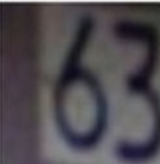
\includegraphics[width=16px]{chapter1/svhn6.png}
        
\includegraphics[width=16px]{chapter1/svhn8.png}                                                                                                                                                          \\
        \midrule
        MNIST                                                                         & \multirow{2}{*}{\textbf{99.17\%}}                 & \multirow{2}{*}{78.08\%}          & \multirow{2}{*}{31.50\%}          \\
        
\includegraphics[width=16px]{chapter1/mnist3.png}
        
\includegraphics[width=16px]{chapter1/mnist6.png}
        
\includegraphics[width=16px]{chapter1/mnist8.png}                             &                                                   &                                   &                                   \\
        USPS                                                                          & \multirow{2}{*}{57.10\%}                          & \multirow{2}{*}{\textbf{95.42\%}} & \multirow{2}{*}{26.94\%}          \\
        
\includegraphics[width=16px]{chapter1/usps3.png}
        
\includegraphics[width=16px]{chapter1/usps6.png}
        
\includegraphics[width=16px]{chapter1/usps8.png}                              &                                                   &                                   &                                   \\
        SVHN                                                                          & \multirow{2}{*}{61.92\%}                          & \multirow{2}{*}{64.28\%}          & \multirow{2}{*}{\textbf{89.52\%}} \\
        
\includegraphics[width=16px]{chapter1/svhn3.png}
        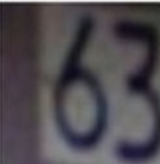
\includegraphics[width=16px]{chapter1/svhn6.png}
        
\includegraphics[width=16px]{chapter1/svhn8.png}                              &                                                   &                                   &                                   \\
        \bottomrule
    \end{tabular}
    \caption{Precisión que se obtiene al aplicar un modelo LeNet5 entrenado con otros conjuntos de datos de dígitos.}
    \label{tab:lenet-distintos-datasets}
\end{table}

En conclusión, debido a que la escritura de los números en los telegramas puede variar de elección en elección y a que
los datos de entrenamiento no son suficientes para una clasificación precisa en este contexto, se necesita recurrir a
técnicas más complejas de entrenamiento que permitan al modelo adaptarse a diferentes dominios. La adaptación de
dominio es una técnica que busca reducir el efecto del sesgo de los datos y hacer que el modelo sea más robusto ante
las variaciones en la escritura de los números. En la actualidad, no existen trabajos publicados que comparen
diferentes técnicas de adaptación de dominio para la digitalización de telegramas en Argentina, lo que sugiere una
oportunidad para investigar y desarrollar modelos más efectivos para este propósito.

\section{Objetivos}

El objetivo general de esta tesis es poder clasificar los dígitos de los votos en las elecciones legislativas de la
provincia de Santa Fe del año 2021 mediante adaptación de dominio de forma que el modelo generalice y no dependa de un
etiquetado de los datos. El enfoque se centrará en explorar y comparar diferentes técnicas de adaptación de dominio con
el fin de lograr un modelo robusto que pueda generalizar en diferentes contextos y escenarios electorales. Con esto se
contribuye a mejorar la transparencia y eficiencia en los procesos electorales en Argentina y sentar las bases para el
desarrollo de soluciones similares para el resto de las provincias y la nación.

Los objetivos específicos para lograr el objetivo planteado son los siguientes:

\begin{itemize}
    \item Armar el proceso de extracción, transformación y carga (ETL) de los telegramas, con el propósito de segmentar y limpiar
          de manera efectiva los dígitos. Los datos utilizados serán obtenidos de fuentes oficiales del estado
          argentino\footnote{\href{https://op.elecciones.gob.ar/telegramas/generales2021/}{https://op.elecciones.gob.ar/telegramas/generales2021/}.}.
          En el anexo \ref{anexo:telegrama} se adjunta un ejemplo de uno de ellos.
    \item Entrenar distintas arquitecturas de redes convolucionales mediante técnicas de adaptación de dominio.
    \item Analizar y evaluar las métricas relevantes para seleccionar el mejor modelo.
    \item Detectar oportunidades de mejora en el proceso eleccionario respecto a los telegramas.
\end{itemize}

\section{Estructura de la tesis}

Esta tesis se encuentra organizado con la siguiente estructura:

\begin{itemize}
    \item Capítulo 2: Marco teórico del reconocimiento de dígitos, redes neuronales, aprendizaje por transferencia y adaptación
          de dominio.
    \item Capítulo 3: Metodología del trabajo realizado sobre los telegramas de las elecciones de Santa Fe. Proceso de
          extracción, transformación y limpieza de los mismos. Diseño experimental y métricas de evaluación.
    \item Capítulo 4: Análisis de resultados. Análisis de métricas, espacios latentes obtenidos y errores observados.
    \item Capítulo 5: Conclusiones del trabajo, mejoras planteadas y futuras investigaciones.
\end{itemize}